% Options for packages loaded elsewhere
\PassOptionsToPackage{unicode}{hyperref}
\PassOptionsToPackage{hyphens}{url}
%
\documentclass[
  11pt,
  a4paper,11pt]{article}
\usepackage{amsmath,amssymb}
\usepackage{iftex}
\ifPDFTeX
  \usepackage[T1]{fontenc}
  \usepackage[utf8]{inputenc}
  \usepackage{textcomp} % provide euro and other symbols
\else % if luatex or xetex
  \usepackage{unicode-math} % this also loads fontspec
  \defaultfontfeatures{Scale=MatchLowercase}
  \defaultfontfeatures[\rmfamily]{Ligatures=TeX,Scale=1}
\fi
\usepackage{lmodern}
\ifPDFTeX\else
  % xetex/luatex font selection
\fi
% Use upquote if available, for straight quotes in verbatim environments
\IfFileExists{upquote.sty}{\usepackage{upquote}}{}
\IfFileExists{microtype.sty}{% use microtype if available
  \usepackage[]{microtype}
  \UseMicrotypeSet[protrusion]{basicmath} % disable protrusion for tt fonts
}{}
\makeatletter
\@ifundefined{KOMAClassName}{% if non-KOMA class
  \IfFileExists{parskip.sty}{%
    \usepackage{parskip}
  }{% else
    \setlength{\parindent}{0pt}
    \setlength{\parskip}{6pt plus 2pt minus 1pt}}
}{% if KOMA class
  \KOMAoptions{parskip=half}}
\makeatother
\usepackage{xcolor}
\usepackage[margin=1in]{geometry}
\usepackage{graphicx}
\makeatletter
\def\maxwidth{\ifdim\Gin@nat@width>\linewidth\linewidth\else\Gin@nat@width\fi}
\def\maxheight{\ifdim\Gin@nat@height>\textheight\textheight\else\Gin@nat@height\fi}
\makeatother
% Scale images if necessary, so that they will not overflow the page
% margins by default, and it is still possible to overwrite the defaults
% using explicit options in \includegraphics[width, height, ...]{}
\setkeys{Gin}{width=\maxwidth,height=\maxheight,keepaspectratio}
% Set default figure placement to htbp
\makeatletter
\def\fps@figure{htbp}
\makeatother
\setlength{\emergencystretch}{3em} % prevent overfull lines
\providecommand{\tightlist}{%
  \setlength{\itemsep}{0pt}\setlength{\parskip}{0pt}}
\setcounter{secnumdepth}{5}
% Load essential packages early
\RequirePackage{mathtools}

% Avoid microtype issues by disabling problematic features
\PassOptionsToPackage{protrusion=false, expansion=false}{microtype}

% Essential packages for graphics, tables, and code
\usepackage{graphicx}    % For including images
\usepackage{booktabs}    % For professional-looking tables
\usepackage{caption}     % For better figure and table captions
\usepackage{listings}    % For code formatting

% Hyperlinks setup - load last
\usepackage{hyperref}
\hypersetup{
    colorlinks=true,
    linkcolor=blue,
    citecolor=blue,
    urlcolor=blue,
    pdfborder={0 0 0},    % Removes boxes around links for a cleaner look
    bookmarksopen=true,   % Opens bookmarks by default
    bookmarksdepth=2      % Controls depth of bookmarks
}

% Listings configuration for code chunks
\lstset{
    basicstyle=\ttfamily\small, % Small font for better readability in code blocks
    columns=flexible,           % Adjust column spacing automatically
    breaklines=true,            % Allow line breaks in code
    showspaces=false,           % Hide spaces for cleaner appearance
    showstringspaces=false,     % Hide spaces within strings
    keepspaces=true,            % Keeps whitespace for code alignment
    frame=single,               % Adds a simple frame around code blocks
    rulecolor=\color{gray},     % Frame color for consistency
    xleftmargin=1em,            % Adds padding to the left for better readability
    xrightmargin=1em,           % Adds padding to the right
    backgroundcolor=\color[gray]{0.95}, % Subtle background for code blocks
    numbers=left,               % Line numbers on the left
    numberstyle=\tiny\color{gray}, % Styling for line numbers
    lineskip=-1pt               % Reduce line spacing within code blocks
}
\usepackage{geometry}
\geometry{a4paper, margin=1in}
\usepackage{lscape}
\usepackage{setspace}
\onehalfspacing
\usepackage{parskip}
\setlength{\parindent}{0pt}
\hypersetup{colorlinks=true, linkcolor=blue, urlcolor=blue, citecolor=blue}
\usepackage{amsmath}
\usepackage{amssymb}
\usepackage{mathtools}
\usepackage{bm}
\usepackage{caption}
\usepackage{hyperref}
\usepackage{geometry}
\usepackage{setspace}
\usepackage{booktabs}
\usepackage{longtable}
\usepackage{colortbl}
\usepackage{array}
\usepackage{anyfontsize}
\usepackage{multirow}
\ifLuaTeX
  \usepackage{selnolig}  % disable illegal ligatures
\fi
\usepackage{bookmark}
\IfFileExists{xurl.sty}{\usepackage{xurl}}{} % add URL line breaks if available
\urlstyle{same}
\hypersetup{
  pdftitle={MTHM506 - Statistical Data Modelling: Individual Project},
  pdfauthor={James R Lewis},
  hidelinks,
  pdfcreator={LaTeX via pandoc}}

\title{MTHM506 - Statistical Data Modelling: Individual Project}
\author{James R Lewis}
\date{March 2025}

\begin{document}
\maketitle

{
\setcounter{tocdepth}{2}
\tableofcontents
}
\textbf{Declaration of AI Assistance}: I have used OpenAI's ChatGPT tool
in creating this report.

AI-supported/AI-integrated use is permitted in this assessment. I
acknowledge the following uses of GenAI tools in this assessment:

\begin{enumerate}
\def\labelenumi{\arabic{enumi}.}
\tightlist
\item
  I have used GenAI tools to check and debug my code.
\item
  I have used GenAI tools to proofread and correct grammar or spelling
  errors.
\item
  I have used GenAI tools to give me feedback on a draft.
\end{enumerate}

I declare that I have referenced use of GenAI outputs within my
assessment in line with the University referencing guidelines.

\newpage

\begin{table}[!t]
\caption{\label{tab:table-1}Table 1: Summary Statistics of Socio-Economic Covariates and TB Rate} 
\caption*{
{\large \textbf{Summary Statistics of Socio-Economic Covariates and TB Rate}}
} 
\fontsize{9.8pt}{11.7pt}\selectfont
\begin{tabular*}{1\linewidth}{@{\extracolsep{\fill}}lrrrrrrr}
\toprule
Covariate & {\bfseries Mean} & Std Dev & {\bfseries Min} & 25th Percentile & {\bfseries Median} & 75th Percentile & {\bfseries Max} \\ 
\midrule\addlinespace[2.5pt]
Indigenous & 0.84 & 3.53 & 0.01 & 0.06 & 0.11 & 0.24 & 50.65 \\ 
Illiteracy & 14.80 & 9.30 & 2.34 & 6.68 & 11.52 & 22.84 & 41.14 \\ 
Urbanisation & 71.96 & 16.53 & 22.34 & 58.45 & 72.66 & 86.16 & 99.93 \\ 
Density & 0.62 & 0.17 & 0.42 & 0.52 & 0.58 & 0.66 & 1.68 \\ 
Poverty & 44.37 & 19.37 & 5.92 & 26.23 & 42.60 & 63.91 & 77.88 \\ 
Poor Sanitation & 16.45 & 12.51 & 0.05 & 6.39 & 13.91 & 25.00 & 58.43 \\ 
Unemployment & 6.93 & 2.56 & 1.13 & 5.15 & 6.78 & 8.40 & 20.44 \\ 
Timeliness & 47.67 & 21.47 & 0.00 & 31.29 & 48.36 & 62.58 & 96.69 \\ 
TB Rate & 23.54 & 15.42 & 0.00 & 13.52 & 20.11 & 28.94 & 117.73 \\ 
\bottomrule
\end{tabular*}
\end{table}

\begin{figure}
\centering
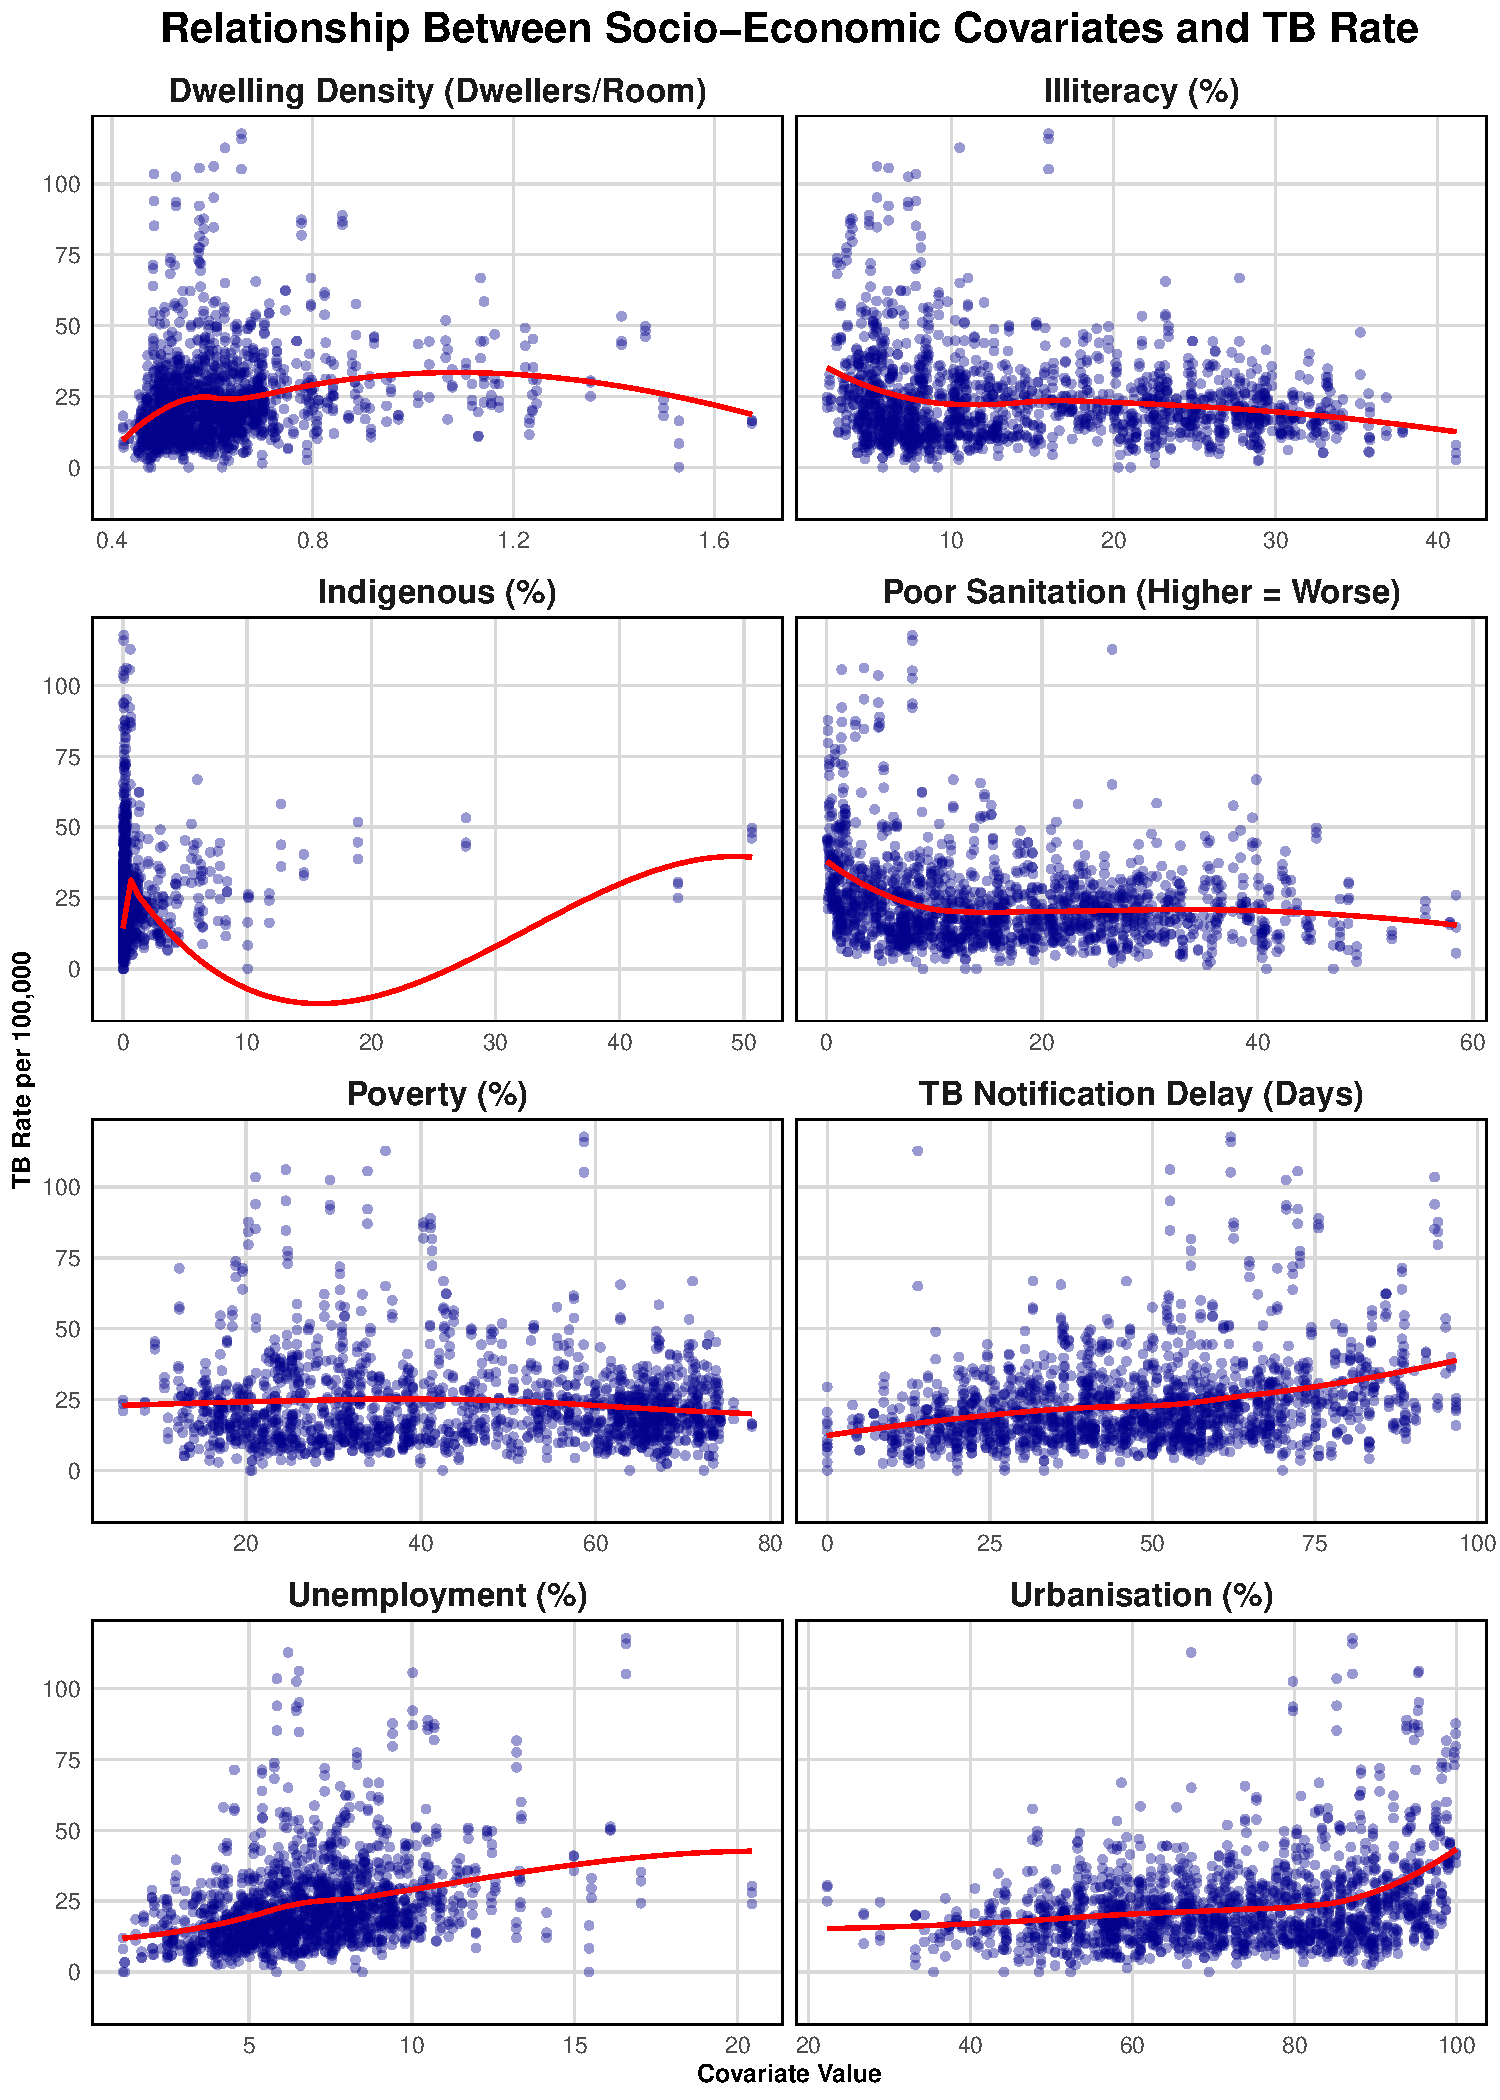
\includegraphics{Project_clean_files/figure-latex/Figure-1-1.pdf}
\caption{Relationship Between Socio-Economic Covariates and TB Rate per
100,000 Population.}
\end{figure}

\end{document}
